\chapter{Organisation du travail}

\section{Répartition des tâches}

Comme le projet peut être découpé en plusieurs blocs qui peuvent être
développés de manière presque indépendante, nous nous sommes répartis
par équipe de 2 ou 3 sur chaque bloc. Certains blocs nécessitent
cependant une base provenant d’autres blocs pour faire des tests.
Par exemple, la partie IHM aura besoin d’une base de données pour
vérifier que la recherche d’imagettes dans celle-ci se déroule bien.
Nous allons donc commencer par développer des prototypes simplifiés
pour que tout le monde puisse améliorer sa partie.

\paragraph{}
Voici la répartition que nous avons effectuée sur les différents blocs :

\begin{center}
\begin{tabular}{ | l | l | }
\hline
{\textbf{Partie du projet}}             &   {\textbf{Responsables}} \\ \hline
{Préparation des données}               &   {Enzo CRANCE \& Valentin FOUCHER} \\ \hline
{Base de données}                       &   {Corentin GUILLOUX \& Kévin DESPOULAINS} \\ \hline
{Interface Homme-Machine}               &   {Laure DU MESNILDOT \& Charlotte RICHARD} \\ \hline
{Interface avec les reconnaisseurs}     &   {TODO} \\ \hline
\end{tabular}
\end{center}

\paragraph{}
Cette répartition des tâches permet à chaque équipe de spécifier plus en détail
sa partie, et donc de pouvoir estimer plus précisément le temps que prendra le
développement. Nous espérons donc avoir un rapport de planification précis qui
nous permettra d’anticiper d’éventuelles réorganisations d’équipes en fonction
des différentes charges de travail.

\section{Organisation temporelle}

Certains membre du groupe partent en mobilité en Janvier (Kévin DESPOULAINS,
Corentin GUILLOUX, et Gaël GENDRON). Notre premier objectif est donc de
concevoir la base et la documentation de chaque partie avant leur départ.
Nous allons donc anticiper la phase de développement en la débutant dès à
présent. Le diagramme de Gantt précédemment établi se trouve donc modifié de
cette manière :

\paragraph{}
\begin{mdframed}[frametitle={Gantt + légende}, innerbottommargin=10]
\begin{center}
%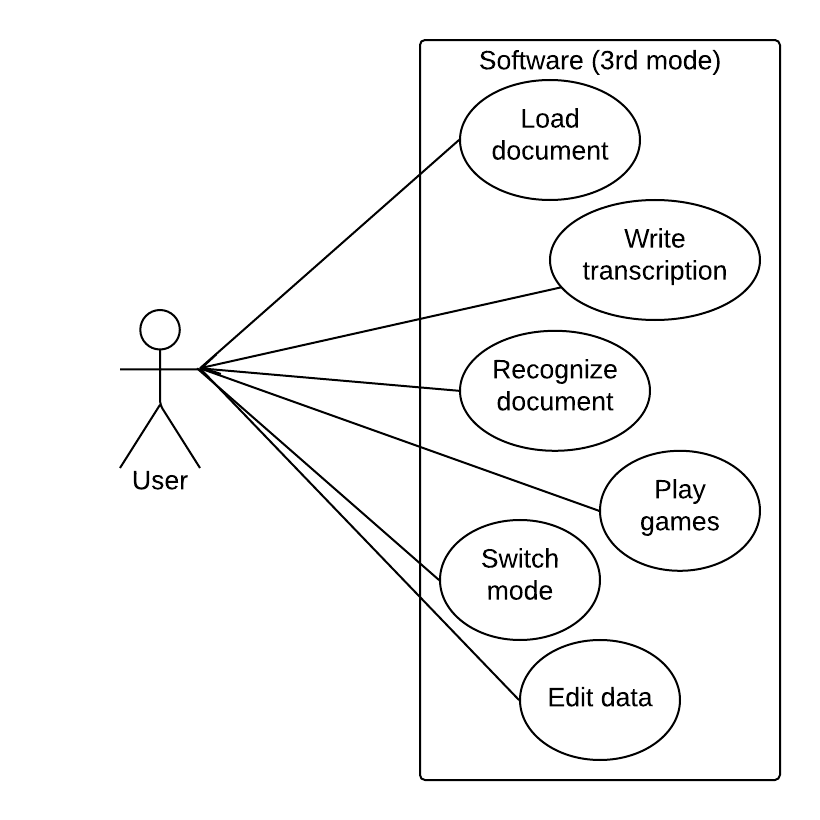
\includegraphics[scale=0.6]{Usecase_3.png}
\end{center}
\end{mdframed}

\section{Délivrables ?}

\begin{mdframed}[frametitle={Figure N : LOT 1 - X}, innerbottommargin=10]
\begin{center}
\begin{tabular}{ | l | l | }
\hline
{\textbf{Règles}}   &   {\textbf{Description}} \\ \hline
{XX\_1}              &   {Règle XX\_1} \\ \hline
\end{tabular}
\end{center}
\end{mdframed}

Formats
PR\_FO\_1 : Permettre de traiter le format PiFF
PR\_FO\_2 : Permettre de traiter le format GEDI
Traitement
PR\_TR\_1 : Fonction de détection de lignes intégrée au logiciel
PR\_TR\_2 : Permettre un découpage des images en lignes
PR\_TR\_3 : Localiser les paragraphes
PR\_TR\_4 : Permettre un découpage des images en paragraphes
Représentation des données
PR\_RE\_1 : Associer les images à leur transcription
PR\_RE\_2 : Associer la vérité terrain à une transcription
PR\_RE\_3 : Permettre de générer une vérité terrain si besoin, grâce à un reconnaisseur

GEN\_ERGO : Ergonomie du logiciel
GEN\_EVOL : Logiciel évolutif

INT\_FMT : Fournir des données intelligibles par le reconnaisseur
INT\_RES : Récupérer les résultats
GEN\_EVOL : Changer de reconnaisseur (pouvoir installer n’importe quel reconnaisseur)

INT\_MOD : L’utiliser dans plusieurs modes
-Apprentissage
-Evaluation
-Production